\chapter{DESAIN DAN IMPLEMENTASI}
\label{chap:design-and-implementation}

% Ubah bagian-bagian berikut dengan isi dari desain dan implementasi

Bab ini menjelaskan desain dan implementasi dari sistem yang telah dibuat.
Seperti yang terlihat pada Gambar \ref{fig:block-diagram}, terdapat 2 diagram blok utama. Di bagian kiri adalah diagram blok untuk mode \textit{RECORD} dan diagram blok kanan adalah untuk mode \textit{PLAY}.
Pada mode \textit{RECORD}, dimulai dengan citra manusia yang menjadi input ke estimasi pose untuk mendapatkan \textit{keypoint} manusia.
Setelah itu, melakukan konversi sudut antara 2 \textit{keypoint} menjadi nilai servo sehingga dapat menggerakkan servo-servo robot untuk menirukan gerakan manusia serta menyimpannya untuk mode \textit{PLAY}.
\begin{figure}[ht]
  \centering
  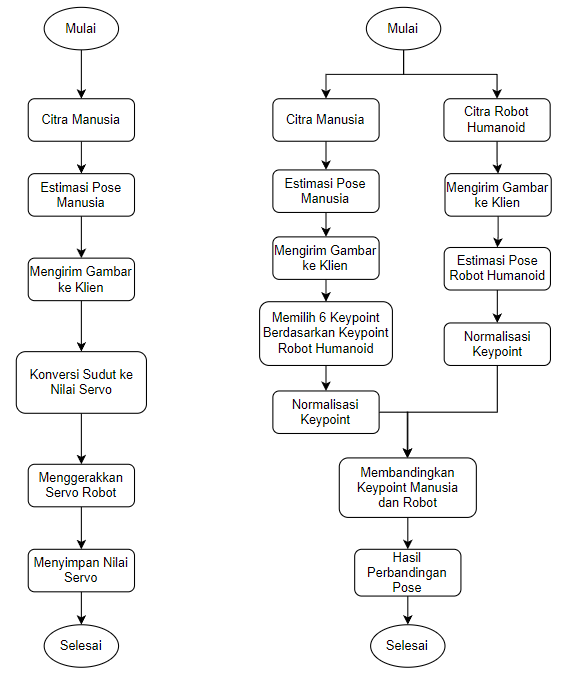
\includegraphics[scale=1.1]{gambar/diagram-block.png}
  \caption{Blok Diagram dari Alur Pengerjaan.}
  \label{fig:block-diagram}
\end{figure}
Di sisi lain, input pada mode \textit{PLAY} terdiri dari 2 yaitu citra manusia dan citra robot \textit{humanoid}.
Kemudian, dilakukan estimasi pose untuk kedua citra tersebut. Sebelum melakukan normalisasi \textit{keypoint}, dilakukan pemilihan 6 \textit{keypoint} manusia berdasarkan \textit{keypoint} robot \textit{humanoid}.
Terakhir, membandingkan \textit{keypoint} tersebut serta mendapatkan hasilnya.
Pada bagian berikutnya, setiap blok akan dijelaskan secara lebih rinci. Perlu diperhatikan bahwa mungkin ada penjelasan yang digabung jika kita menggunakan teknik yang sama untuk blok yang berbeda.
Misalnya, blok yang mengirimkan citra manusia ke klien dan blok yang mengirimkan citra robot ke klien akan digabung menjadi hanya mengirimkan citra ke klien.


\section{Citra Input}
\label{sec:input-image}

Citra input yang dimasukkan ke dalam dua model (manusia dan robot \textit{humanoid}) memiliki ukuran 640x480 piksel dengan saluran RGB.
Perangkat yang digunakan untuk mendapatkan citra adalah Logitech C920 Webcam. Kami menggunakan \textit{library} OpenCV untuk membuka kamera dan mengambil citra.


\section{Estimasi Pose Manusia}
\label{sec:estimasi-pose-manusia}

Dikarena sudah banyaknya model estimasi pose untuk manusia yang tersedia, kami tidak perlu melakukan pelatihan ulang dan hanya membandingkannya untuk mencari model terbaik melalui referensi dari beberapa makalah.
Metrik evaluasi berdasarkan paper dan hasil deteksi setiap model akan ditunjukkan pada Bab \ref{chap:resultsandiscussion}, namun untuk waktu inferensi akan dicoba pada NUC i5.
Model-model yang dibandingkan adalah OpenPose, MediaPipe Pose, dan YOLO-pose. Input untuk model-model ini adalah citra RGB lalu outputnya adalah lokasi \textit{keypoint} manusia.

\section{Mengirim Citra ke Klien}
\label{sec:send-image-to-client}

Program utama kami menggunakan website untuk berinteraksi dengan pengguna karena fleksibilitasnya pada berbagai \textit{platform}, tampilan website dapat dilihat pada Gambar \ref{fig:websiteview}. 
Akan ada klien Javascript dan Server Python yang berkomunikasi melalui \emph{socketio}.
Server akan mengirimkan citra manusia ke klien sehingga kita dapat menyesuaikan posisi kita di depan kamera. Hal ini dilakukan agar robot dapat mengambil seluruh pose manusia.
\begin{figure}[ht]
  \centering
  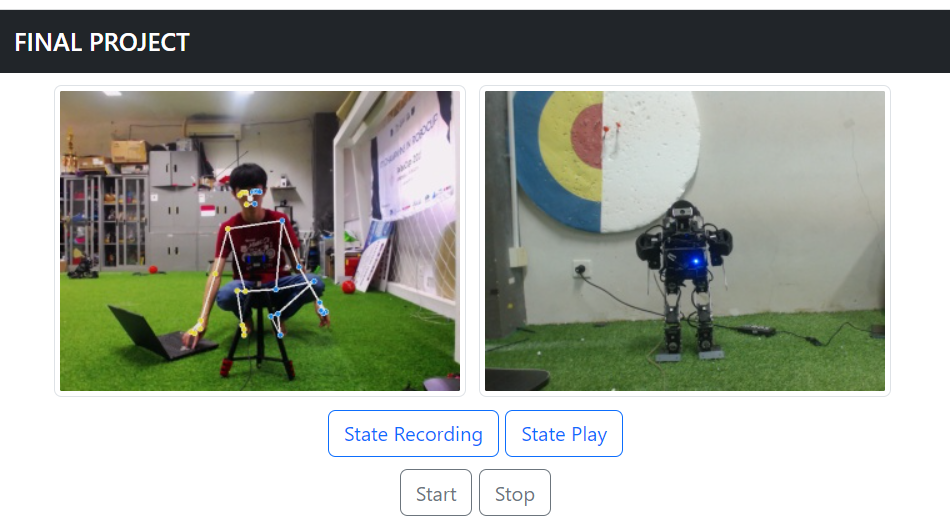
\includegraphics[scale=0.7]{gambar/web.png}
  \caption{Tampilan Website.}
  \label{fig:websiteview}
\end{figure}
Program utama ini terbagi menjadi dua mode, yaitu mode \textit{RECORD} dan mode \textit{PLAY}. Pada mode \textit{RECORD}, manusia berperan sebagai pelatih dan memberikan serangkaian gerakan yang akan ditiru oleh robot \textit{humanoid} serta gerakan tersebut akan disimpan oleh robot untuk digunakan di mode \textit{PLAY} nantinya.
Sementara itu, pada mode \textit{PLAY}, robot bertindak sebagai pelatih dan memperagakan serangkaian gerakan sesuai yang disimpan pada mode \textit{RECORD}. Manusia akan meniru gerakan robot selagi robot juga menyimpan citra manusia dan citra robot lalu membandingkannya nanti.

Setelah mendapatkan \textit{keypoint} manusia, server akan memvisualisasikan hasil deteksinya dan mengirimkan sebagai buffer ke klien.
Di sisi klien, kami menggunakan \textit{library ReactJS}. Terdapat empat tombol: tombol \textit{RECORD}, \textit{PLAY}, \textit{START}, dan \textit{STOP}. Tombol \textit{RECORD} dan \textit{PLAY} mengindikasikan mode dalam program utama, sementara tombol \textit{START} dan \textit{STOP} memberitahu kapan mode dimulai atau dihentikan.
Setelah mengklik tombol, tombol tersebut akan berubah warna untuk menunjukkan bahwa tombol tersebut sudah ditekan.
Selain itu, terdapat dua citra yang menampilkan citra manusia dan robot. Sebenarnya, pada mode \textit{RECORD} hanya ada satu citra (citra manusia), sedangkan pada mode \textit{PLAY} terdapat 2 citra (citra manusia dan citra robot).
Klien dan server berkomunikasi melalui port 5555, di mana server dapat mengirim citra ke klien dan klien dapat mengirim beberapa data kembali ke server seperti mode saat ini dan waktu untuk memulai atau menghentikan mode.
Kami menggunakan fungsi \emph{useEffect} untuk mengindikasi jika terdapat perubahan pada variabel tertentu dan melakukan sesuatu seperti mengonversi citra dari buffer menjadi \textit{string} untuk ditampilkan pada tag HTML.


\section{Konversi Sudut ke Nilai Servo}
\label{sec:convert-angle-to-servo-value}

Bagian ini dan Bagian \ref{sec:move-robot-servo} dijalankan ketika tombol \textit{RECORD} dan \textit{START} ditekan pada website, sehingga klien mengirimkan informasi ini ke server dan server melakukan perhitungan.
Untuk dapat menggerakkan tubuh bagian atas robot sesuai dengan gerakan manusia, kita perlu mendapatkan sudut antara 2 \textit{keypoint} menggunakan fungsi \emph{arc tangent} dengan input koordinat \textit{keypoint} \emph{{x, y}}
DiKarenakan kami menggunakan MediaPipe Pose untuk mendeteksi \textit{keypoint} manusia berdasarkan hasil dan pembahasan di Bagian \ref{sec:humanmodelcomparison}, outputnya adalah titik yang ternormalisasi, jadi harus dilakukan pengkalian koordinat x dan y dengan lebar dan tinggi gambar masing-masing untuk mendapatkan nilai piksel yang sebenarnya.
Selanjutnya, kita membagi nilai \textit{keypoint} y dengan nilai \textit{keypoint} x serta menginputkan hasilnya ke fungsi \emph{arc tangent}, seperti yang ditunjukkan dalam Persamaan \ref{eq:arctan}.
\begin{equation}
  \label{eq:arctan}
  angle = \arctan \left(\frac{Y_2 - Y_1}{X_2 - X_1}\right)
\end{equation}

Ada empat sudut yang ingin diperoleh, yaitu sudut dari bahu ke siku (kanan dan kiri) dan juga siku ke pergelangan tangan (kanan dan kiri) agar robot dapat meniru gerakan bagian atas tubuh manusia.
Jika kita melihat MediaPipe Pose Landmark pada Gambar \ref{fig:mediapipe-landmark}, 6 \textit{keypoint} yang menjadi perhatian adalah 11, 12 untuk bahu, 13, 14 untuk siku, 15, dan 16 untuk pergelangan tangan.
Kita mendapatkan nilai sudut bahu kanan dengan memasukkan landmark 14 sebagai argumen kedua dan landmark 12 sebagai argumen pertama dari fungsi \emph{arc tangent}. Hal yang sama juga berlaku untuk mendapatkan nilai sudut bahu kiri dengan memasukkan landmark 13 dan 11 secara berurutan.
Hal ini sedikit berbeda untuk mendapatkan sudut siku karena kita ingin sudutnya relatif terhadap sudut bahu dengan mengurangi sudutnya dari sudut bahu.
Kami juga memberlakukan batasan untuk setiap sudut untuk menjaga keamanan servo dan menghindari benturan dengan tubuh robot atau servo lainnya seperti yang terlihat pada Tabel \ref{tb:robot-servos}.
\begin{longtable}{ccc}
  \caption{Limitasi Servo Robot.}
  \label{tb:robot-servos}\\
  \hline
  \rowcolor[HTML]{C0C0C0}
  \textbf{Joint Angle} & \textbf{Motion} & \textbf{Range (deg)} \\
  \hline
  LShoulderRoll       & Left shoulder joint right and left    & -110 to 30  \\
  RShoulderRoll       & Right shoulder joint right and left   & -30 to 110 \\
  LElbowPitch           & Left Elbow joint front and back       & -120 to 10  \\
  RElbowPitch           & Left Elbow joint front and back       & -10 to 120  \\
  \hline
\end{longtable}


\section{Menggerakkan Servo-servo Robot}
\label{sec:move-robot-servo}

Program untuk menggerakkan servo robot berada di tempat yang sama dengan program untuk \textit{server}. Program utama kami menggunakan ROS2 dengan bahasa Python. Untuk dapat menjalankan program \textit{server} dan program ROS2 secara bersamaan, kami membutuhkan \textit{thread} terpisah sehingga program \textit{server} tidak menghalangi ROS2.
Dalam \textit{framework} ROS2, setiap \textit{package} memiliki fungsionalitasnya masing-masing. Pada kesempatan ini, kami membagi tugas untuk menggerakkan servo robot menjadi 2 \textit{package}. Yang pertama bernama \emph{motion matching} di mana program server dan konversi sudut menjadi nilai servo terjadi, yang satunya lagi adalah \emph{tachimawari}, sebuah \textit{package} yang menyediakan \textit{management library} sendi DYNAMIXEL untuk proyek ROS 2.
Nama paket ini berasal dari kata bahasa Jepang yang berarti \textit{motion}. Setiap \textit{package} memiliki sebuah \textit{node} dengan nama \textit{package} itu sendiri seperti yang terlihat pada Gambar \ref{fig:relation-node-record-mode}.
Hubungan antar node ini dapat dilihat melalui grafik rqt atau \textit{ROS2 client interfaces}, tetapi kami memilih grafik rqt karena lebih visual.
\begin{figure}[ht]
  \centering
  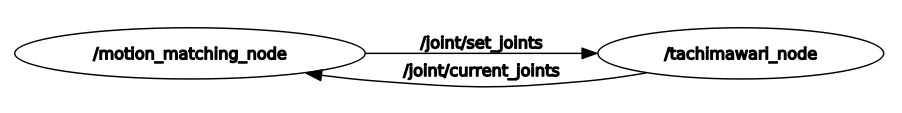
\includegraphics[scale=0.62]{gambar/rqt_without_akushon.png}
  \caption{Hubungan Antar \textit{Node} pada Mode \textit{RECORD}.}
  \label{fig:relation-node-record-mode}
\end{figure}

Setiap \textit{node} berkomunikasi satu sama lain melalui topik. Terdapat 2 topik dalam mode \textit{RECORD}, yaitu \verb|joint/set_joints| dan \verb|joint/current_joints|.
Setelah mendapatkan sudut servo yang diinginkan dari bagian sebelumnya, kita hanya perlu mem-\textit{publish} ke \emph{tachimawari node} dan \textit{node} tersebut akan menggerakkan servonya. Di dalam \emph{motion matching node}, terdapat sebuah \emph{publisher} yang mem-\textit{publish} sudut servo ke topik \verb|joint/set_joints| setelah proses deteksi dan
perhitungan selesai dilakukan, serta terdapat \emph{subscriber} pada \emph{tachimawari node} yang mendengarkan pada topik yang sama untuk mengumpulkan data yang di-\textit{publish} oleh \emph{publisher}. Topik \verb|joint/set_joints| menggunakan antarmuka seperti yang terlihat pada potongan kode \ref{lst:set-joint-msg}, di mana terdapat variabel \verb|control_type| dengan tipe data \textit{integer} dan sebuah array dengan tipe \textit{Joint}, setiap \textit{Joint} terdiri dari \textit{id} dan \textit{position} seperti pada potongan kode \ref{lst:joint-msg}.
\begin{lstlisting}[
  language={},
  caption={\textit{Joint msg}.},
  label={lst:joint-msg}
]
uint8 id
float32 position
\end{lstlisting}

\begin{lstlisting}[
  language={},
  caption={\textit{SetJoints msg}.},
  label={lst:set-joint-msg}
]
int8 control_type 4
Joint[] joints
\end{lstlisting}

Di dalam \verb|tachimawari_node| terdapat \verb|joint_node| yang mempublikasikan nilai sendi saat ini setiap 8ms (akan digunakan pada bagian berikutnya) dan memiliki \emph{subscriber} yang mendengarkan sendi yang ingin kita gerakkan.
Untuk dapat menggerakkan servonya ke nilai yang diinginkan, kita harus mengaktifkan \emph{torque} dari semua servo terlebih dahulu. Kemudian kita membuat sebuah perintah dalam bentuk \textit{array} yang berisi \textit{id} servo dan nilai yang diinginkan atau nilai target kita (16 \textit{byte}) yang dibagi menjadi 2 * 8 \textit{byte}.
Sebagai contoh, nilai target kita adalah 512 (dalam bentuk biner sama dengan \verb|00000010 00000000|), pesan yang kita kirim adalah 2 (\verb|00000010|) dan 0 (\verb|00000000|). Hal ini dapat kita peroleh dengan melakukan operasi \textit{bitwise AND} dan \textit{bitwise right shif}t. Operasi \textit{bitwise AND} dilakukan antara nilai target dan \verb|0xFF|, yang direpresentasikan sebagai (\verb|00000000 11111111|) dalam bentuk biner.
Karena \verb|0xFF| memiliki 0 \textit{bit} di \textit{byte} yang lebih tinggi dan 1 \textit{bit} di \textit{byte} yang lebih rendah, hasil dari operasi tersebut adalah \textit{byte} yang lebih rendah dari nilai target. Di sisi lain, operator \textit{bitwise right shift} digunakan untuk menggeser \textit{bit-bit} servo target 8 posisi ke kanan. Menggeser \textit{bit} ke kanan sejauh 8 posisi secara efektif menghilangkan \textit{byte} yang lebih rendah, sehingga hanya \textit{byte} yang lebih tinggi yang tersisa dalam hasilnya.
Hal ini juga berlaku ketika kita menerima nilai posisi servo saat ini, servo juga mengirimkan data dalam bentuk dua \textit{byte} (\textit{byte} yang lebih rendah dan \textit{byte} yang lebih tinggi) dan kita perlu menggabungkan kedua \textit{byte} tersebut untuk merekonstruksi nilai 16-\textit{bit} yang mewakili posisi servo saat ini. Hal ini dapat dicapai dengan melakukan operasi \textit{left shift} pada \textit{byte} yang lebih tinggi.
Menggeser 8 \textit{bit} ke kiri secara efektif memindahkannya ke posisi \textit{byte} yang lebih tinggi. Setelah itu, operasi \textit{bitwise OR} menggabungkan \textit{byte} yang lebih tinggi yang telah digeser dengan \textit{byte} yang lebih rendah. Operasi ini menggabungkan kedua \textit{byte} tersebut untuk membentuk nilai 16-\textit{bit} yang mewakili posisi saat ini.


\section{Menyimpan Nilai Servo}
\label{sec:save-servo-value}

Pada bagian sebelumnya, kita telah membahas sedikit mengenai \emph{publisher} dalam \textit{package} \emph{tachimawari} yang mempublikasikan nilai setiap sendi saat ini dari robot melalui topik \verb|joint/current_joints|.
Terdapat juga \emph{subscriber} di dalam \verb|motion_matching| \textit{node} yang mengambil data tersebut, dan \textit{timer} ROS2 yang dijalankan setiap 0.5 detik untuk menyimpan \emph{current joints} saat ini dalam format JSON seperti pada potongan kode \ref{lst:json-save-joints}, sehingga robot dapat bergerak sesuai dengan gerakan yang diperagakan oleh manusia.
Format JSON yang disediakan mewakili objek data terstruktur yang menggambarkan tindakan atau urutan gerakan tertentu. Terdapat \textit{array} "\textit{poses}" yang berisi beberapa objek \textit{pose}, masing-masing mewakili konfigurasi \emph{joint} tertentu selama \textit{action} tersebut.
Setiap objek pose mencakup sub-objek "\textit{joints}", yang mencantumkan berbagai \emph{joint} dan nilai-nilai yang terkait. Misalnya, \verb|"left_ankle_pitch"| memiliki nilai 25, \verb|"left_ankle_roll"| diatur menjadi 0, dan seterusnya. Nilai-nilai ini mewakili posisi atau sudut dari \emph{joint} yang bersangkutan.
Setiap objek pose juga memiliki bagian "\textit{name}" untuk mengidentifikasi pose tersebut. Bagian "\textit{pause}" menentukan durasi jeda antara pose ini dan pose berikutnya, sedangkan "\textit{speed}" menunjukkan seberapa cepat pose ini akan dieksekusi.
Terakhir, bagian \verb|"start_delay"| menandakan jeda sebelum tindakan dimulai, dan bagian \verb|"stop_delay"| menandakan jeda setelah tindakan selesai sebelum robot berhenti. Secara keseluruhan, terdapat 20 servo pada robot, sehingga dalam file JSON yang sebenarnya, setiap sub-objek "\textit{joint}" memiliki 20 item dengan nama-nama \emph{joint} yang sesuai.
\begin{lstlisting}[
  language={},
  caption={Format JSON untuk Menyimpan Nilai Servo.},
  label={lst:json-save-joints}
]
{
  "poses": [
    {
      "joints": {
        "left_ankle_pitch": 25,
        "left_ankle_roll": 0,
      },
      "name": "pose name",
      "pause": 0,
      "speed": 0.003
    },
  ],
  "start_delay": 0,
  "stop_delay": 0
}
\end{lstlisting}


\section{Estimasi Pose Robot \textit{Humanoid}}
\label{sec:humanoid-robot-pose-estimation}

Penjelasan ini ditujukan untuk blok diagram kanan dari Gambar \ref{fig:block-diagram} atau bisa juga disebut sebagai mode \textit{RECORD}. Perbedaan antara mode \textit{PLAY} dan \textit{RECORD} terletak pada jumlah kamera yang digunakan.
Jadi akan ada dua kamera, satu kamera untuk merekam gerakan manusia (terletak di kepala robot) dan satu lagi untuk merekam gerakan robot (terletak dari sisi manusia menghadap robot), dengan jarak antara kamera sekitar 1 - 1,5 meter, seperti yang ditunjukkan pada Gambar \ref{fig:pose-comparison-side}.
Pada mode \textit{PLAY}, server mengirimkan dua gambar agar kita dapat mengetahui dan menyesuaikan posisi manusia dan robot dalam kamera. Karena adanya \textit{delay} jaringan yang besar saat mengirimkan dua gambar berukuran 320x240 piksel sekaligus, ketika tombol \textit{START} ditekan,
server tidak mengirimkan gambar ke klien lagi, robot melakukan serangkaian gerakan yang disimpan dalam file JSON sebelumnya dengan berkomunikasi melalui \textit{package} ROS2 lainnya, sambil menyimpan kedua gambar tersebut. Setelah itu, ketika tombol \textit{STOP} ditekan, server akan membandingkan pose antara keduanya.
\begin{figure}[ht]
  \centering
  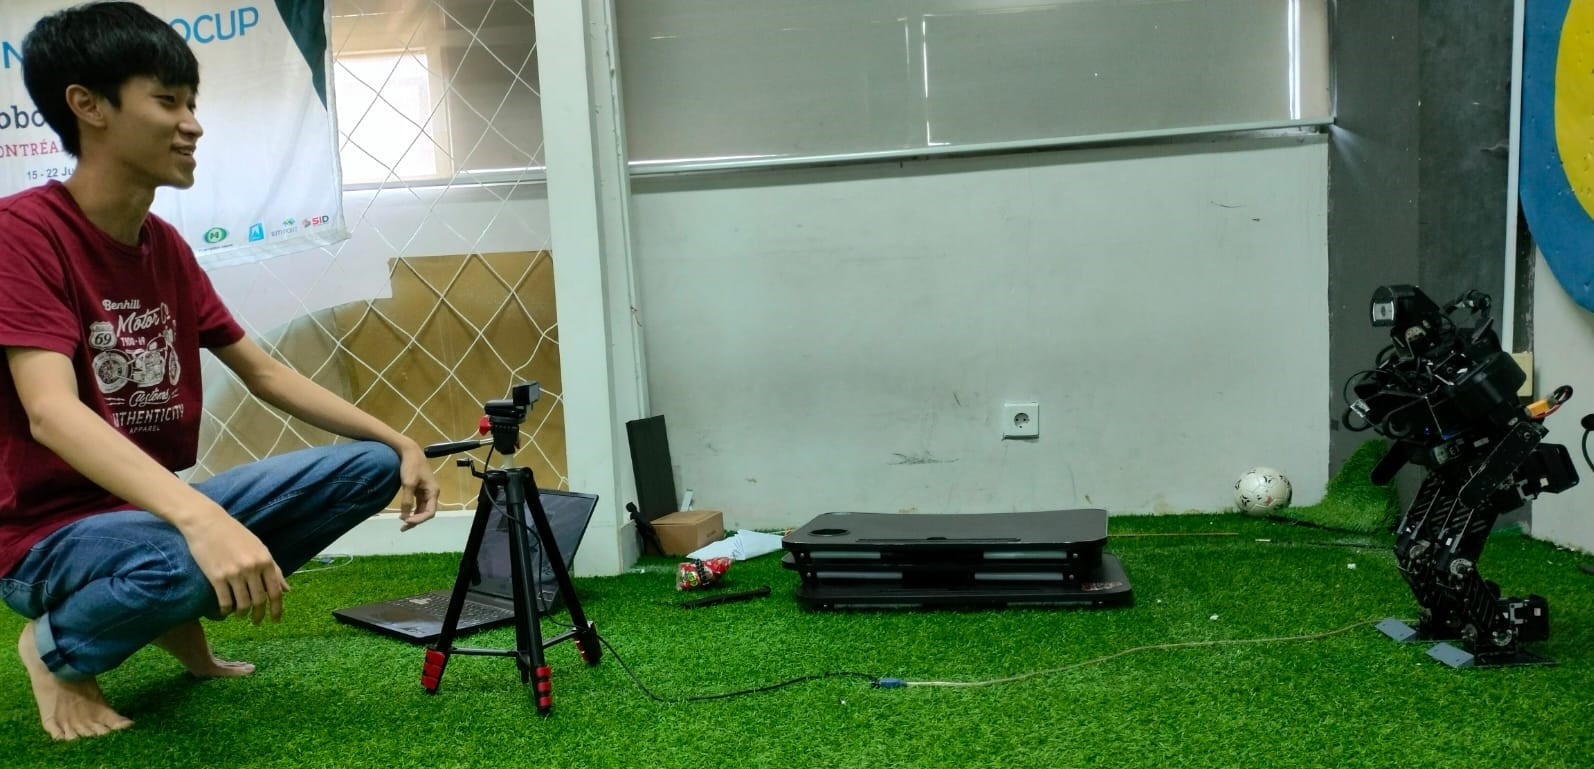
\includegraphics[scale=0.3]{gambar/pose-comparison.jpeg}
  \caption{Membandingkan Pose dari Sisi Samping.}
  \label{fig:pose-comparison-side}
\end{figure}

Untuk dapat menggerakkan servo-servo robot sesuai dengan data yang tersimpan dalam JSON, diperlukannya sebuah \textit{package} yang disebut \emph{akushon}. \emph{Akushon} adalah paket yang terkait dengan gerakan robot. Asal usul nama paket ini berasal dari kata bahasa Jepang yang berarti \textit{action}.
Seperti yang dijelaskan pada Bagian \ref{sec:move-robot-servo}, setiap paket memiliki sebuah \textit{node} dengan nama \textit{package}-nya sendiri dan berkomunikasi satu sama lain melalui topik, seperti yang ditunjukkan pada Gambar \ref{fig:relation-node-play-mode}. Terdapat 3 topik pada mode \textit{PLAY}: topik \verb|joint/set_joints| dan topik \verb|joint/current_joints| yang digunakan oleh \verb|akushon_node|, \verb|tachimawari_node|, dan \verb|motion_matching_node|,
serta topik \verb|action/run_action| yang digunakan antara \verb|aku| \verb|shon_node| dan \verb|motion_matching_node|.
Penjelasan mengenai bagaimana menggerakkan servo-servo robot dan mendapatkan nilai servo saat ini melalui topik \verb|joint/set_joints| dan \verb|joint/current_joints| terdapat pada Bagian \ref{sec:move-robot-servo}.
Sementara itu, topik \verb|action/run_action| digunakan untuk mengirimkan data pose dalam file JSON dari \textit{package} \emph{motion matching} ke \textit{package} \emph{akushon}. Pada \textit{package} \emph{akushon}, terdapat sebuah \textit{interpolator} yang melakukan iterasi pada setiap pose dalam file JSON, memperoleh setiap nilai servo, dan mengirimkannya ke \textit{package} \emph{tachimawari}.
\begin{figure}[ht]
  \centering
  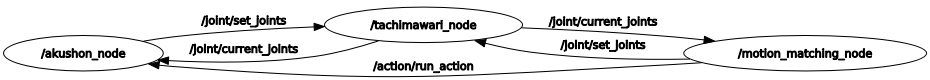
\includegraphics[scale=0.64]{gambar/rqt_akushon.png}
  \caption{Hubungan Antar \textit{Node} pada Mode \textit{PLAY}.}
  \label{fig:relation-node-play-mode}
\end{figure}

Bagian ini akan langsung membahas estimasi pose untuk robot \textit{humanoid} karena penjelasan mengenai blok sebelumnya telah dijelaskan pada bagian sebelumnya.
Dikarenakan belum banyak model estimasi pose yang khusus untuk robot \textit{humanoid}, kita perlu melakukan pelatihan ulang model atau menggunakan \textit{transfer learning} dari model yang seharusnya ditujukan untuk mengestimasi pose manusia.
Oleh karena itu, sub-bagian berikut akan menjelaskan langkah-langkah untuk melatih estimasi pose pada robot \textit{humanoid}.

\subsection{Membuat Dataset Baru}
\label{subsec:make-new-dataset}

Dataset baru ini merupakan kombinasi antara \textit{HumanoidRobotPose} dataset milik NimbRo dan dataset milik kami sendiri. 
Dataset dari NimbRo mencakup robot tunggal dan multi robot dalam 1 gambar dan diambil dalam kondisi nyata \textit{RoboCup}. 
Mereka mengumpulkan data dari video YouTube Liga \textit{Humanoid RoboCup}, video internal mereka sendiri, dan file \textit{ROS bags}. 
Secara keseluruhan, dataset mereka memiliki lebih dari 1.5 ribu gambar yang berasal dari 23 video dengan sekitar 2.3 ribu jumlah robot. 
Gambar-gambar ini mencakup robot berukuran \textit{teen} dan \textit{adult} serta mengandung lebih dari sepuluh jenis robot yang berbeda \parencite{amini2021}.
Namun, robot-robot dalam dataset kami hanya berukuran \textit{kid} dan hadir dalam konfigurasi tunggal atau maksimal dua robot. Gambar-gambar dalam dataset kami berasal dari video yang diambil di laboratorium kami. Lalu video-video tersebut dijadikan beberapa gambar dan dipilih video yang tidak buram.
Sebelum dilakukan penggabungan, kami perlu memperbaiki format dataset dari NimbRo terlebih dahulu. Hal ini karena setelah kami memvisualisasikan beberapa data mereka, kami menemukan bahwa \textit{bounding box} pada bagian "\textit{annotations}" tertukar (lebar dan tingginya tertukar).
Setelah kami memperbaiki format dataset mereka dan menggabungkannya dengan dataset kami, dataset yang baru terbentuk memiliki sekitar 2.1 ribu gambar.
Sekitar 20 persen dari dataset tersebut digunakan untuk skoring dan validasi.

Terkait dengan \textit{annotation tools}, terdapat banyak pilihan termasuk offline dan online. Kami telah mencoba beberapa di antaranya seperti Dataloop, V7labs, atau Supervisely yang direkomendasikan oleh NimbRo. Namun, ketika kami mencoba untuk meng-\textit{export} dataset ke dalam format COCO,
terjadi kegagalan (misalnya tidak dapat di-\textit{impor} atau dapat di-\textit{impor} tetapi hasil JSON pada bagian anotasi tidak ada). Oleh karena itu, kami memutuskan untuk menggunakan coco-annotator, ala anotasi gambar berbasis web yang dirancang untuk fleksibilitas dan efisiensi dalam memberikan label pada gambar untuk membuat data pelatihan.
Terkait jumlah keypoints pada setiap robot, kami mengikuti dataset dari NimbRo. Terdapat enam \textit{keypoint} termasuk \textit{head}, \textit{trunk}, \textit{hands}, dan \textit{feet}. Kami tetap berpegang pada ide tersebut karena kami ingin mencoba performa dan waktu inferensi model dengan jumlah \textit{keypoint} yang lebih sedikit terlebih dahulu, dan jika hasilnya memuaskan, kami akan meningkatkan jumlah \textit{keypoint} di kemudian hari.

\subsection{Melatih Estimasi Pose untuk Robot \textit{Humanoid}}
\label{subsec:training-robot}

Semua proses pelatihan dalam penelitian ini utamanya dilakukan pada komputer DGX-A100 dan ditulis dalam bahasa pemrograman Python. Konfigurasi spesifikasinya dijelaskan pada Tabel \ref{tb:dgxa100}.
Dari spesifikasi dasar ini, kami dialokasikan suatu kontainer \textit{Jupyter notebook} dengan Python dan banyak \textit{library} yang telah terpasang sebelumnya dengan alokasi sumber daya yang dijelaskan pada Tabel \ref{tb:allocatedcontainer}
\begin{longtable}{|c|c|}
  \caption{Spesifikasi DGX-A100.}
  \label{tb:dgxa100}\\
  \hline
  CPU     & Dual AMD Rome 7742, 128 cores total @ 2.25 GHz \\
  \hline
  GPU     & 8 x NVIDIA A100 80 GB Tensor Core GPUs  \\
  \hline
  RAM     & 2 TB \\
  \hline
  Storage & 30 TB (8 x 3.84 TB) U.2 NVMe drives \\
  \hline
\end{longtable}

\begin{longtable}{|c|c|}
  \caption{Spesifikasi Kontainer yang Dialokasikan.}
  \label{tb:allocatedcontainer}\\
  \hline
  GPU     & 1/8 NVIDIA A100 GPU \\
  \hline
  GPU RAM & 10 GB  \\
  \hline
  CPU RAM & 8 GB \\
  \hline
  Storage & 100 GB  \\
  \hline
\end{longtable}

\subsubsection{Model NimbRo}
\label{subsubsec:training-nimbro-model}

Hyperparameter yang digunakan untuk melatih model NimbRo mengikuti deskripsi dalam makalah mereka.
Model ini dilatih menggunakan \textit{optimizer} AdamW dengan \textit{learning rate} 10\textsuperscript{-4},
ukuran batch 16, dan \textit{weight decay} 10\textsuperscript{-4} untuk total 200 epoch.
Perlu diperhatikan bahwa encoder diinisialisasi dengan ResNet yang telah dilatih sebelumnya pada dataset ImageNet.
Kami juga melakukan augmentasi data yang mencakup \textit{scaling} dan translasi selama pelatihan \parencite{amini2021}.
\textit{Flip horizontal} acak dan rotasi tidak digunakan karena dalam kasus kami, hal tersebut akan membuat hasil pelatihan menjadi lebih buruk.

Program utama untuk pelatihan telah disediakan oleh mereka pada file \emph{main.py} menggunakan \textit{framework} PyTorch, kita hanya perlu menjalankannya pada Jupyter Notebook atau Terminal dan menyesuaikan argumen sesuai kebutuhan kita.
Dalam skrip mereka, terdapat argumen dengan nama \verb|config| yang merujuk pada file di mana kami menyimpan semua hyperparameter, jumlah epoch, nama dataset untuk pelatihan dan pengujian, dan lain-lain.
Argumen lainnya memberitahu kita tentang tempat menyimpan hasil pelatihan dan lokasi dari dataset.
\newpage
\lstinputlisting[
  language={},
  caption={Contoh \textit{config} file YAML untuk pelatihan Model NimbRo.},
  label={lst:confignimbro}
]{files/train_nimbro.yaml}
File \ref{lst:confignimbro} merupakan contoh \textit{config} file YAML untuk pelatihan NimbRo. Ini bukan merupakan versi lengkap, tetapi disitu telah dicantumkan bagian-bagian yang sering diubah selama proses pelatihan.
\verb|"SEED"| diatur menjadi 42, memastikan terjadinya proses acak. \verb|"DEVICE"| ditentukan sebagai \textit{"cuda"}, menandakan penggunaan GPU untuk komputasi.
\verb|"BATCH_SIZE"| diatur menjadi 16, yang berarti 16 sampel data akan diproses bersamaan dalam setiap iterasi pelatihan. Jika kita membuat nilai \emph{batch size} lebih besar, diperlukan juga lebih banyak memori untuk menyimpan data input dan gradien selama pelatihan.
Jika memori yang tersedia terbatas, meningkatkan ukuran \textit{batch} melebihi kapasitas memori dapat menyebabkan \textit{error out-of-memory} atau memperlambat proses pelatihan.
Namun, ukuran batch yang lebih besar dapat mempercepat proses pelatihan karena lebih banyak sampel diproses secara paralel. Hal ini juga mempengaruhi kemampuan generalisasi dari model.
Ukuran batch yang lebih kecil cenderung mempunyai lebih banyak \textit{stochasticity} selama pelatihan, yang dapat berfungsi sebagai bentuk regularisasi dan membantu mencegah overfitting. Sebaliknya, ukuran batch yang lebih besar dapat menghasilkan proses optimasi yang lebih halus, dengan potensi konvergensi lebih cepat tetapi risiko overfitting sedikit meningkat.
\verb|"NUM_WORKERS"| bernilai 2, menunjukkan bahwa dua proses pekerja akan digunakan untuk memuat dan memproses data.

Proses pelatihan akan berjalan selama 200 epoch sesuai dengan \verb|"NUM_EPOCHS"| yang ditentukan. Semakin banyak epoch, model akan mengalami lebih banyak iterasi dan pembaruan, memungkinkannya untuk menyempurnakan representasi yang dipelajari dan menyesuaikan parameter berdasarkan data pelatihan.
Hal ini dapat menghasilkan peningkatan performa model karena model mendekati solusi optimal dan mencapai akurasi yang lebih tinggi baik pada data pelatihan maupun validasi. Namun, juga perlu berhati-hati terhadap risiko \textit{overfitting}. \textit{Overfitting} terjadi ketika model menjadi terlalu khusus pada data pelatihan dan gagal untuk menggeneralisasi dengan baik pada data yang belum pernah dilihat sebelumnya.
Meningkatkan jumlah epoch tanpa teknik regularisasi yang tepat dapat meningkatkan risiko ini. Model dapat mulai menghafal data pelatihan daripada belajar pola yang digeneralisasi sehingga dapat menghasilkan performa yang buruk pada data baru. Selain itu, melatih untuk jumlah epoch yang lebih besar membutuhkan waktu yang lebih lama.
\verb|"PRINT_FREQ"| bernilai 100, artinya informasi yang relevan dengan proses pelatihan akan dicetak setiap 100 iterasi.

Bagian \verb|"DATASET"| berisi pengaturan terkait dataset yang digunakan untuk pelatihan.
\verb|"DA| \verb|TASET.TRAIN"| menentukan nama folder untuk dataset pelatihan, dan \verb|"DATASET.TEST"| menunjukkan nama folder untuk dataset validasi. \verb|"NUM_KEYPOINTS"| diatur menjadi 6, yang menandakan jumlah \textit{keypoint} atau landmark dalam dataset, sementara \verb|"NUM_LIMBS"| diatur menjadi 5, mewakili jumlah hubungan antara keypoints (\textit{limb}).
\verb|"MAX_NUM_DETECTIONS"| diatur menjadi 10, menunjukkan jumlah maksimum robot dalam satu gambar. Parameter \verb|"SIGMA"| diatur menjadi 2.0, yang digunakan dalam pembentukan \textit{heatmap}. Untuk augmentasi, \verb|"FLIP"| diatur menjadi 0.0, yang berarti tidak akan ada \textit{horizontal flipping} pada data input. \verb|"TRANSLATE"| diatur menjadi 0.4, memungkinkan data untuk ditranslasi hingga 40\% dari ukuran aslinya.
Parameter \verb|"SCALE"| mewakili rentang \textit{scaling} yang diterapkan pada data input, dengan skala minimum 0.5 dan skala maksimum 1.5. \verb|"ROTATION"| diatur menjadi 0, menunjukkan bahwa tidak akan ada rotasi yang diterapkan. Selain itu, \verb|"INPUT_SIZE"| diatur menjadi [384, 384], mewakili ukuran input yang diinginkan dari model, sedangkan \verb|"OUTPUT_SIZE"| diatur menjadi [192, 192], menunjukkan ukuran output model.

Untuk menghitung \textit{loss}, mereka menggunakan \textit{mean square error} (MSE) antara \textit{heatmap} yang diprediksi dan \textit{heatmap ground truth} baik untuk \textit{keypoints} dan \textit{limb}.
Fungsi loss ini secara langsung membandingkan prediksi koordinat \textit{keypoint} dengan koordinat \textit{ground truth} dengan cara mengambil rata-rata selisih kuadrat antara koordinat yang diprediksi dan koordinat target.
Akhirnya, total \textit{loss} adalah jumlah dari \textit{loss keypoint} dan \textit{loss limb} \parencite{amini2021}.

\subsubsection{YOLO-pose}
\label{subsubsec:training-yolo-pose}

Sebelum memulai proses pelatihan, kita harus mengubah format dataset yang baru dari COCO ke YOLO. Berbeda dengan format COCO, format YOLO memberikan nilai \textit{visibility flag} keypoint 2 jika \textit{keypoint} yang terlihat atau terhalang, tetapi jika \textit{keypoint} berada di luar bidang pandang, nilainya menjadi nol.
Namun, format COCO mendefinisikan \textit{visibility flag} sebagai v=0: tidak dilabeli, v=1: dilabeli tetapi tidak terlihat, dan v=2: dilabeli dan terlihat. Jadi, kita mengubah definisi v=1 dan v=2 menjadi v=2 dalam format YOLO dan mempertahankan v=0. Seperti yang terlihat dalam Pseudocode \ref{lst:change-keypoint-format}, di mana kita membuat fungsi bernama \verb|change_keypoint_format| yang memiliki 2 argumen masukan dan fungsi tersebut mengembalikan \textit{keypoint} baru dengan format YOLO.
Selain perbedaan format \textit{keypoint}, format \textit{bounding-box} diantara keduanya juga berbeda. COCO mendefinisikan \textit{bounding-box} sebagai berikut: x (kiri atas), y (kiri atas), lebar, dan tinggi. Di sisi lain, format \textit{bounding-box} dalam YOLO adalah: x (pusat), y (pusat), lebar, dan tinggi, dan semuanya perlu dinormalisasi.
Oleh karena itu, kita perlu menambahkan 1/2 lebar ke x, 1/2 tinggi ke y seperti yang terlihat dalam Pseudocode \ref{lst:change-bbox-format} dan menormalisasinya melalui perkalian x dan y yang baru dengan 1/lebar dan 1/tinggi secara berturut-turut.
\newpage
\lstinputlisting[
  language={},
  caption={Mengganti Format \textit{Keypoint} dari COCO ke YOLO.},
  label={lst:change-keypoint-format}
]{program/change-keypoint.txt}

\lstinputlisting[
  language={},
  caption={Mengganti Format \textit{Bounding Box} dari COCO ke YOLO.},
  label={lst:change-bbox-format}
]{program/bbox-norm.txt}

Hyperparameter untuk melatih YOLO-pose mengikuti deskripsi yang ada pada GitHub mereka dengan file \emph{hyp.pose.yaml}.
Kami menggunakan \textit{optimizer} SGD dengan \textit{cosine scheduler}. \textit{Learning rate} diatur menjadi 10\textsuperscript{-2}, ukuran batch 16,
dan \textit{weight decay} sebesar 5\textsuperscript{-4} untuk total 100 epoch. Terdapat juga augmentasi data seperti augmentasi skala ([0.5, 1.5]),
translasi [-10, 10], augmentasi mozaik dengan probabilitas 1, dan berbagai augmentasi warna.
Seperti pada bagian sebelumnya, program utama untuk pelatihan telah disediakan menggunakan \textit{framework} PyTorch juga, tetapi program ini ditujukan untuk manusia dengan 17 \textit{keypoint}.
Jika menjalankannya langsung dengan dataset kami yang memiliki 6 keypoints, akan muncul \textit{error}. Oleh karena itu, kode perlu diubah sedikit agar proses pelatihan dapat berjalan.

\textit{Loss} keseluruhan untuk YOLO-pose adalah jumlah dari \textit{classification loss}, \textit{bounding box loss}, \textit{keypoint loss}, dan \textit{keypoints confidence loss} dengan batasan tertentu seperti yang terlihat dalam Persamaan \ref{eq:overall-loss-yolo}.
Hyperparameter yang dipilih untuk menjaga keseimbangan antara \textit{loss} pada skala yang berbeda adalah $\lambda_{cls} = 0.5$, $\lambda_{box} = 0.05$, $\lambda_{kpts} = 0.1$, dan $\lambda_{kpts_conf} = 0.5$.
Perlu dicatat bahwa, \textit{loss} pada lokasi (\emph{i,j}) berlaku untuk anchor k\textsuperscript{th} pada skala s jika \textit{ground truth bounding box} cocok dengan anchor tersebut \parencite{maji2022yolopose}.
\begin{equation}
  \label{eq:overall-loss-yolo}
  \mathcal{L}_{total} = \sum_{s,i,j,k} (\lambda_{cls}\mathcal{L}_{cls} + \lambda_{box}\mathcal{L}_{box} + \lambda_{kpts}\mathcal{L}_{kpts} + \lambda_{kpts_conf}\mathcal{L}_{kpts_conf})
\end{equation}

Daripada menggunakan \textit{distance-based loss} untuk deteksi \textit{bounding box}, sebagian besar detektor objek modern mengoptimalkan variasi IoU \textit{loss} seperti GIoU, DIoU, atau CIoU karena \textit{loss} ini terpengaruh terhadap skala dan secara langsung mengoptimalkan ukuran evaluasi itu sendiri.
Mereka menggunakan CIoU \textit{loss} untuk \textit{bounding box}. Untuk \textit{ground truth bounding box} yang sesuai dengan anchor ke-k di lokasi (i, j) dan skala s, \textit{loss} didefinisikan sebagai berikut \parencite{maji2022yolopose}.
\begin{equation}
  \label{eq:bbox-loss-yolo}
  \mathcal{L}_{box}(s,i,j,k) = (1 - CIoU(Box_{gt}^{s,i,j,k}, Box_{pred}^{s,i,j,k}))
\end{equation}

Secara konvensional, pendekatan bottom-up berbasis \textit{heatmap} menggunakan \textit{loss} L1 untuk mendeteksi \textit{keypoints}. Namun, \textit{loss} L1 mungkin tidak selalu cocok untuk mendapatkan OKS optimal untuk metrik evaluasi karena tidak mempertimbangkan skala objek atau jenis \textit{keypoints}.
Oleh karena itu, mereka menggunakan \textit{loss} OKS, mereka memperluas ide \textit{loss} IOU dari \textit{bounding box} menjadi \textit{keypoints}. OKS diperlakukan sebagai IOU dalam hal \textit{keypoints}. OKS dihitung untuk setiap \textit{keypoints} secara terpisah dan kemudian dijumlahkan untuk memberikan \textit{loss} OKS akhir
atau \textit{loss} IOU \textit{keypoints} seperti Persamaan \ref{eq:keypoint-loss-yolo}, di mana $\delta(V_n > 0)$ = \textit{visibility flag} untuk setiap \textit{keypoints} \parencite{maji2022yolopose}.
\begin{equation}
  \label{eq:keypoint-loss-yolo}
  \mathcal{L}_{kpts}(s,i,j,k) = 1 - \frac{\sum_{n=1}^{N_{kpts}} exp\left( \frac{d_n^2}{2s^2k_n^2} \right) \delta(V_n > 0) }{\sum_{n=1}^{N_{kpts}} \delta(V_n > 0)}
\end{equation}

Untuk mendapatkan \textit{loss} dari \textit{keypoint confidence}, mereka menggunakan \textit{Loss} Binary Cross-Entropy. Parameter ini menunjukkan apakah sebuah \textit{keypoint confidence} ada atau tidak untuk objek tersebut. Di sini, \textit{visibility flags} untuk \textit{keypoint} digunakan sebagai \textit{ground truth}.
$p_{kpts}^n$ = prediksi \textit{confidence} untuk \textit{keypoint} n\textsuperscript{th} \parencite{maji2022yolopose}.
\begin{equation}
  \label{eq:keypoint-confident-loss-yolo}
  \mathcal{L}_{kpts_conf}(s,i,j,k) = \sum_{n=1}^{N_{kpts}} BCE(\delta(V_n > 0), p_{kpts}^n)
\end{equation}

\subsubsection{Keypoint RCNN}
\label{subsubsec:training-rcnn}

Pelatihan Keypoint RCNN dilakukan langsung pada \textit{Jupyter Notebook} menggunakan \textit{framework} PyTorch juga.
Sebelum memulai proses pelatihan, kita perlu mengonversi format dataset terlebih dahulu.
Sebenarnya, format Keypoint RCNN hampir sama dengan format YOLO (setiap gambar memiliki label sendiri), tetapi perbedaannya terletak pada \textit{bounding box}.
Di mana format \textit{bounding box} adalah titik kiri atas dan titik kanan bawah. Kita dapat memperoleh titik kanan bawah dengan menambahkan lebar ke koordinat x dan tingginya ke koordinat y.

Proses pelatihan dimulai dengan memuat dataset dan menentukan teknik augmentasi yang akan gunakan. Kami menggunakan \emph{albumentations library} dari Python untuk mengaugmentasi dataset kami.
Kami menerapkan augmentasi kecerahan, kontras, dan rotasi.
Sebelum kami mendeklarasikan model RCNN menggunakan \textit{torchvision library}, kita juga perlu mendifinisikan anchor yang akan menjadi argumen input.
Pada dasarnya, \emph{AnchorGenerator class} dalam PyTorch memiliki 3 ukuran yang berbeda (128, 256, 512) dan 3 rasio aspek yang berbeda (0.5, 1.0, 2.0).
Kami telah memperluas parameter tersebut, \verb|sizes| menjadi (32, 64, 128, 256, 512), yang berarti akan dihasilkan kotak anchor dengan ukuran yang berbeda-beda. Ukuran ini mewakili dimensi perkiraan (dalam piksel) dari objek yang akan diidentifikasi oleh algoritma.
Argumen \verb|aspect_ratios| menentukan rasio aspek kotak anchor. Hal ini mengacu pada rasio lebar terhadap tinggi kotak anchor.
Argumen \verb|aspect_ratios| diatur menjadi (0.25, 0.5, 0.75, 1.0, 2.0, 3.0, 4.0), yang berarti anchor dengan rasio aspek ini akan dihasilkan. Dengan mengkombinasikan 2 argumen tersebut, dihasilkan anchor yang beragam.
Kotak-kotak anchor ini kemudian dibandingkan dengan \textit{ground truth bounding box} dari objek dalam data pelatihan untuk menentukan lokasi objek.
Perhatikan bahwa argumen \verb|num classes| diatur menjadi dua karena kelas pertama adalah latar belakang (background) dan objeknya adalah kelas kedua.
Dalam pelatihan ini, kami menggunakan \textit{optimizer} SGD dengan \textit{learning rate} 10\textsuperscript{-3}, ukuran batch 3, dan \textit{weight decay} 5\textsuperscript{-4} untuk 50 epoch.

Total \textit{loss} untuk Keypoint RCNN adalah jumlah \textit{loss} untuk \textit{classification}, \textit{bounding box}, dan \textit{keypoint} seperti yang terlihat dalam Persamaan \ref{eq:overall-loss-rcnn}.
Keypoint RCNN menggunakan \textit{Cross-Entropy Loss} untuk menghitung \textit{classification loss} dan \textit{keypoints loss}, serta \textit{smooth L1 loss} untuk \textit{bounding box}.
Untuk deteksi \textit{keypoint}, fungsi \textit{loss} yang digunakan adalah \textit{Mean Squared Error} (MSE) loss atau varian lainnya, yaitu \textit{smooth L1 loss}. Fungsi-fungsi \textit{loss} ini membandingkan langsung koordinat yang diprediksi dari \textit{keypoint} dengan koordinat \textit{ground truth}.
Namun, Keypoint RCNN menggunakan \textit{Cross-Entropy Loss} untuk menghitung \textit{keypoint loss}. Fungsi \textit{loss} ini biasanya digunakan untuk masalah klasifikasi multi-kelas. 
Fungsi ini mengharapkan input berupa probabilitas mentah untuk setiap kelas dan memerlukan label target dalam bentuk indeks kelas. Oleh karena itu, tugas \textit{keypoint} diperlakukan sebagai masalah klasifikasi multi-kelas, di mana setiap \textit{keypoint} dianggap sebagai kelas terpisah.
\begin{equation}
  \label{eq:overall-loss-rcnn}
  \mathcal{L}_{total} = \sum (\mathcal{L}_{cls} + \mathcal{L}_{box} + \mathcal{L}_{kpts})
\end{equation}

\subsection{Mencari Model Terbaik untuk Estimasi Pose Robot \textit{Humanoid}}
\label{subsec:finding-best-model-humanoid-robot}

Setelah melatih ulang 3 model pada Bagian \ref{subsec:training-robot}, kami mencoba mencari yang terbaik untuk kasus kami. Kami membandingkannya berdasarkan \emph{AP} (\textit{Average Precision}),
\emph{AR} (\textit{Average Recall}), hasil deteksi, dan waktu inferensi pada perangkat dengan kemampuan komputasi terbatas (misalnya NUC i5).
Tabel perbandingan dan hasil deteksi nyata dari model-model tersebut ada di Bab \ref{chap:resultsandiscussion}.
\lstinputlisting[
  language=Python,
  caption={Pseudocode untuk Mendapatkan Perbedaan Waktu.},
  label={lst:time-difference}
]{program/time-difference.txt}
Untuk mengetahui waktu yang dibutuhkan oleh model untuk melakukan deteksi, kita perlu mengurangi waktu sebelum dan setelah model melakukan deteksi \textit{keypoint} seperti yang ditunjukkan dalam Pseudocode \ref{lst:time-difference}.
Dalam pseudocode ini, fungsi \verb|get_current_time()| digunakan untuk memperoleh waktu saat ini. Proses deteksi \textit{keypoint} dilakukan pada bagian yang ditunjukkan.
Variabel \verb|elapsed_time| dihitung dengan mengurangi waktu mulai dari waktu saat ini. Akhirnya, waktu inferensi dicetak dengan pesan yang sesuai.

Kami juga mencoba mengonversi model kami dari Model PyTorch ke OpenVINO untuk mempercepat waktu inferensi. Sebelum itu, kami mengonversinya ke ONNX terlebih dahulu seperti yang terlihat pada Gambar \ref{fig:pytorch-to-openvino}.
Pertama, kami harus memastikan bahwa model berada dalam mode inferensi dengan memanggil fungsi \emph{eval} dalam kode Python.
Selanjutnya, kami membuat variabel input \textit{dummy}. Pemanggilan fungsi \emph{torch.onnx.export} menjalankan model sekali untuk melacak jalannya eksekusi dan kemudian mengekspor model pada file yang ditentukan.
File onnx yang dihasilkan berisi protokol buffer biner yang berisi struktur jaringan dan parameter model yang diekspor.
Setelah itu, kami menggunakan Model \textit{Optimizer} untuk mengonversi model ONNX menjadi OpenVINO IR dengan presisi FP16. Untuk meng-\textit{instal} Model Optimizer di Python sangatlah sederhana, cukup menjalankan
\emph{pip install openvino-dev} di Terminal dan untuk memverifikasi bahwa paket tersebut terinstal dengan benar dan jalankan perintah \emph{mo -h}. Jika instalasi selesai, kita akan melihat pesan dari Model Optimizer.
Setelah menjalankan perintah tersebut, akan ada sebuah direktori yang berisi tiga file dengan ekstensi \emph{bin}, \emph{mapping}, dan \emph{xml}.
Jika kita ingin menjalankan Model OpenVINO IR di OpenVINO Runtime, pastikan bahwa folder untuk memuat model tersebut mengandung tiga file yang telah disebutkan sebelumnya.

\begin{figure}[ht]
  \centering
  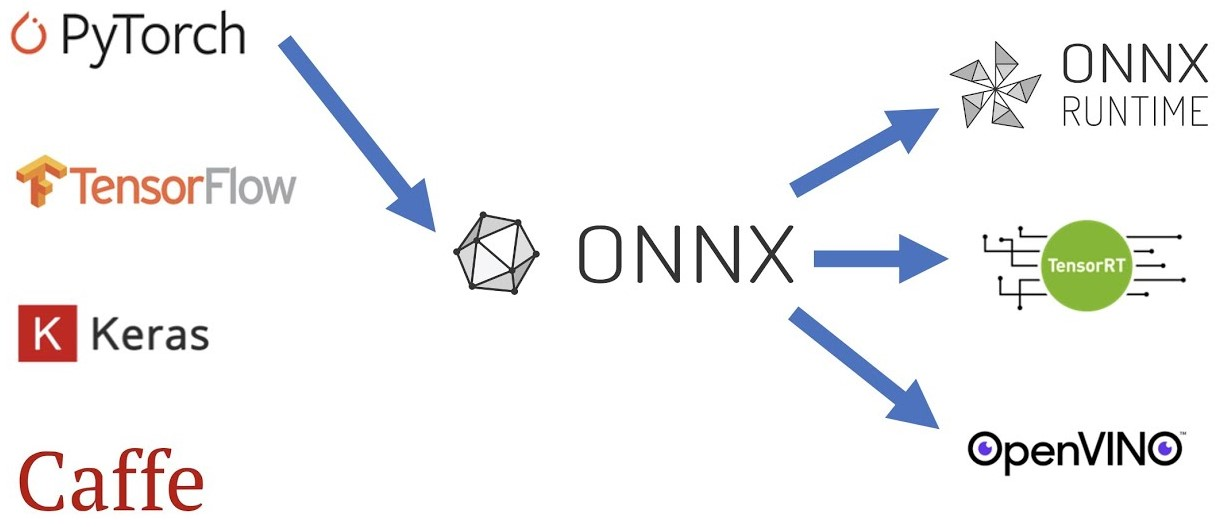
\includegraphics[scale=0.4]{gambar/pytorch-onnx-openvino.jpg}
  \caption{Alur Mengkonversi Model PyTorch ke OpenVINO.}
  \label{fig:pytorch-to-openvino}
\end{figure}


\section{Memilih Enam \textit{Keypoint} Berdasarkan \textit{Keypoint} Robot \textit{Humanoid}}
\label{sec:choose-keypoints}

Perbedaan jumlah \textit{keypoint} yang dihasilkan oleh model antara manusia dan robot membuat kita harus memilih beberapa \textit{keypoint} tertentu pada manusia agar dapat dibandingkan nantinya.
Kami memilih jumlah \textit{keypoint} sebanyak 6 karena mengikuti makalah \parencite{amini2021} yang mencoba untuk mendeteksi 6 \textit{keypoint} pada robot \textit{humanoid} dan mendapatkan hasil yang cukup memuaskan.
Jika kedepannya, jumlah \textit{keypoint} pada robot yang dapat dideteksi oleh model bertambah, maka kita juga akan memilih \textit{keypoint} manusia berdasarkan jumlah tersebut. 
Berdasarkan hasil pengujian, kami memilih Mediapipe untuk manusia dan Keypoint RCNN untuk robot. Mediapipe menghasilkan 33 \textit{keypoint} landmark untuk manusia, sementara Keypoint RCNN hanya menghasilkan 6 \textit{keypoint}.
Oleh karena itu, kita perlu memilih 6 keypoint manusia seperti yang ditunjukkan dalam Pseudocode \ref{lst:choose-human-keypoints}.
Perhatikan bahwa nama \textit{keypoint} dalam kode sesuai dengan nama keypoint pada robot. Pertama, kita mendapatkan semua 33 \textit{keypoint}. Kemudian menghitung \textit{keypoint} yang kita inginkan, seperti \textit{keypoint} kepala yang terletak di antara mata kanan dan kiri.
Untuk mendapatkan landmark mata, kita dapat mengindeks variabel \verb|landmark| sesuai dengan Gambar \ref{fig:mediapipe-landmark}, di mana mata kiri memiliki indeks 2 dan mata kanan memiliki indeks 5. Hal ini juga berlaku untuk landmark lainnya.
\textit{Keypoint} untuk tangan dan kaki diperoleh dengan memilih pergelangan tangan dan pergelangan kaki, di mana landmark[15] dan landmark[16] adalah pergelangan tangan, dan landmark[27] dan landmark[28] adalah pergelangan kaki.
Terakhir, \textit{keypoint} badan terletak di antara \textit{keypoint} bahu dan pinggul. Koordinat x terletak di tengah pinggul. Koordinat y, di sisi lain, terletak pada jarak 1/4 antara pinggul dan bahu dari bawah.
Pertama, kita menentukan titik tengah antara bahu dan pinggul dengan menghitung koordinat sumbu y kanan dan kiri secara individu, seperti yang ditunjukkan dalam Pseudocode \ref{lst:choose-human-keypoints} baris 19 dan 21. Untuk mendapatkan 1/4 jarak antara pinggul dan bahu dari bawah, kita kemudian menghitung titik tengah antara perhitungan sebelumnya dan titik pinggul seperti yang ditunjukkan pada baris 20, 22, dan 24.
Setelah semua perhitungan selesai, kita menyusun semua \textit{keypoint} dalam sebuah array tunggal.

\lstinputlisting[
  language={},
  caption={Memilih \textit{Keypoint} Manusia.},
  label={lst:choose-human-keypoints}
]{program/choose-human-keypoints.txt}

\newpage
\section{Normalisasi \textit{Keypoint}}
\label{sec:keypoint-normalization}

Ketika memikirkan masalah ini, kami melihat bahwa ada banyak ketidakpastian yang perlu ditangani. Misalnya, manusia dan robot \textit{humanoid} dapat berbeda dalam hal tinggi badan, bentuk tubuh, dan lokasi dalam sebuah gambar, misal suatu subjek (manusia atau robot) mungkin berada dekat dengan kamera dan yang lain mungkin berada di kejauhan.
Untuk mendapatkan hasil yang akurat, setiap masalah ini harus diatasi.
Setelah memilih \textit{keypoint}, output model untuk manusia dan robot adalah koordinat dari 6 \textit{keypoint}. Informasi ini dapat digunakan untuk membuat koordinat \textit{keypoint} baru yang dimulai dari (0,0) dalam gambar. Hal ini memecahkan masalah subjek yang muncul di bagian yang berbeda dalam gambar.
\lstinputlisting[
  language={},
  caption={Mendapatkan \textit{Keypoint} Baru.},
  label={lst:new-keypoints}
  ]{program/bbox.txt}

Pada Pseudocode \ref{lst:new-keypoints}, dalam kode tersebut terdapat dua fungsi: \verb|get_min_point| dan \verb|get_new_coords|. Fungsi \verb|get_min_point| menerima input berupa array koordinat \textit{keypoint} dengan bentuk (6,2) dan melakukan iterasi melalui pada tiap item dalam array tersebut.
Fungsi ini melacak nilai minimum x dan y yang ditemui selama iterasi dan mengembalikan array yang berisi koordinat minimum x dan y.
Fungsi \verb|get_new_coords| menerima input berupa array koordinat \textit{keypoint} dan \verb|min_point| (koordinat minimum x dan y) dari perhitungan sebelumnya. Fungsi ini melakukan iterasi pada setiap item dan mengurangkannya dengan nilai minimum x dan y dari setiap koordinat dan mengembalikan hasilnya.

Kami juga melakukan normalisasi pada \textit{keypoint} yang dihasilkan menggunakan normalisasi L2 untuk mengubahnya menjadi vektor satuan seperti yang ditunjukkan pada Gambar \ref{fig:transforming-into-unit-vector}. Hal ini berarti kami mengabaikan ukuran gambar, namun tetap mempertimbangkan arah vektor yang dibentuk oleh pose di dalam gambar tersebut.
Untuk menghitung normalisasi L2, kita gunakan rumus akar kuadrat dari jumlah kuadrat koordinatnya. Perhitungan ini menghasilkan panjang vektor koordinat titik tersebut.
Langkah berikutnya adalah membagi setiap koordinat dengan panjang vektor. Proses normalisasi ini mengubah skala koordinat secara proporsional sambil tetap mempertahankan arah vektor. Selain itu, kita akan mengoptimasi proses tersebut menggunakan \textit{library} NumPy agar dapat menghitung beberapa titik secara simultan.

\begin{figure}[ht]
  \centering
  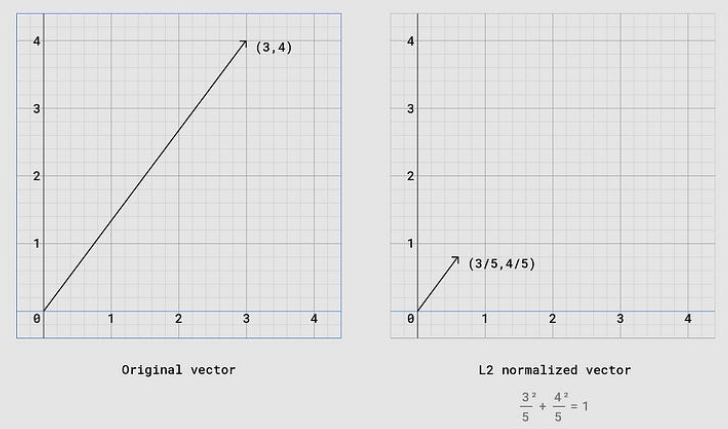
\includegraphics[scale=0.65]{gambar/transform-to-unit-vector.png}
  \caption{Melakukan Transformasi Menjadi Vektor Satuan.}
  \label{fig:transforming-into-unit-vector}
\end{figure}

\section{Membandingkan \textit{Keypoint} Manusia dan \textit{Keypoint} Robot}
\label{sec:comparing-keypoints}

Setelah kita melakukan standarisasi vektor pose, saatnya memilih metode pengukuran kesamaan. Kami memilih kesamaan kosinus karena kami bekerja dengan vektor dan melakukan beberapa perhitungan lanjutan untuk mendapatkan jarak Euclidean yang dapat diinterpretasikan sebagai jarak kosinus (\textit{cosine distance}).
Kesamaan kosinus berkisar dari -1 hingga 1, dengan nilai 1 menunjukkan pose atau vektor yang identik atau berada dalam arah yang sama, nilai 0 menunjukkan ketidakmiripan atau vektor yang hampir ortogonal, dan nilai -1 menunjukkan pose dengan arah yang berlawanan. Sementara itu, jarak kosinus (cosine distance) adalah ukuran ketidakmiripan yang berkisar dari 0 hingga 2.
Menggunakan Persamaan \ref{eq:euclideandistance} akan mengubah skala nilai menjadi rentang 0 hingga 2, sehingga lebih mudah untuk menginterpretasikan hasilnya. Nilai yang lebih besar menunjukkan ketidakmiripan yang lebih besar antara pose. Dalam persamaan tersebut, Fxy dan Gxy adalah dua vektor pose yang akan dibandingkan setelah dilakukan normalisasi L2. Selain itu, Fxy dan Gxy hanya berisi posisi x dan y untuk masing-masing dari 6 keypoints, tidak termasuk \textit{confidence scores}.

\begin{equation}
  \label{eq:cosinesimilarity}
  cosineSimilarity(x,y) = \frac{x \cdot y}{|x||y|}
\end{equation}

\begin{equation}
  \label{eq:euclideandistance}
  D(F_{xy}, G_{xy}) = \sqrt{2 * (1 - cosineSimilarity(F_{xy}, G_{xy}))}
\end{equation}


\section{Hasil Perbanding Pose}
\label{sec:pose-similarity-result}

Hasil perbandingan pose dinyatakan dalam persentase dengan rentang 0 hingga 100. Skor yang lebih tinggi menunjukkan posisi yang lebih mirip diantara manusia dan robot, dan juga sebaliknya.
Untuk mendapatkannya, kita mengalikan hasil \textit{cosine distance} dari Bagian \ref{sec:comparing-keypoints} dengan 100 dan mengurangkan hasil tersebut dari 100.
Setelah mendapatkan hasilnya, kita mengambil rata-rata dan menampilkannya di video di sudut kiri atas. Video ini akan dihasilkan setelah mendeteksi dan membandingkan semua pose.